\section{Introduction}
\label{s_motive}


Nuclear expertise is rapidly expanding around the world as demand for energy increases steadily. Because nuclear energy is clean and carbon-neutral, climate change concerns further tilt the scales making nuclear power appealing to a growing number of countries \cite{mooney_why_2014}.  China is already investing heavily in nuclear power, planning to triple its generating capacity from 19 \gls{GWe} to 58 \gls{GWe} by 2020 \cite{_china_2014}.  As climate change becomes increasingly important with respect to national security, the perception of the risk inherent to nuclear energy is decreasing and states are embracing nuclear energy as a reliable large-scale source of carbon-neutral energy.  However, the expansion of nuclear power amplifies nuclear security concerns, because the same technologies used to produce nuclear fuel can also be exploited in the pursuit of nuclear weapons.  Moreover, in the 70 years since nuclear bombs were dropped on Hiroshima and Nagasaki, the knowledge and technology required to make these weapons has proliferated around the globe \cite{feiveson_unmaking_2014}. There are now nine states that have developed their own nuclear weapons either through indigenous research or transfer of knowledge from existing programs. As nuclear power becomes more ubiquitious, it becomes ever more important to meaningfully decouple the nuclear expertise required for the pursuit of energy from that of nuclear weapons.  


\subsection{Use of Treaties to Curtail Proliferation}

While it has not proven possible to prevent the spread of nuclear knowledge entirely, international treaties have been used in an attempt to minimize it.  The \gls{NPT}, which has been signed by 190 states including the original five nuclear weapons states, has codified a set of rules and norms for allowing the peaceful pursuit of nuclear energy \cite{_treaty_????}.  The \gls{NPT} created the \gls{IAEA}, whose role is to verify compliance with the treaty by periodically inspecting facilities related to nuclear technology.  Other relevant treaties include \gls{CTBT}, which placed a moratorium on testing nuclear weapons, and the \gls{START} in which the \gls{US} and Russia agreed to nuclear arms reductions \cite{_treaty:_????, department_of_State_new_2010}. (The \gls{CTBT} has been signed by 164 states but has not yet entered into force).

These treaties have done much to prevent the spread of nuclear weapons knowledge, but they do not address the weapons production capabilities of states that already posess nuclear weapons.  A potential \gls{FMCT} would place limits on the amount of weapons-grade fissile material that each signatory state could stockpile, possibly including current stockpiles in the case of weapons states.  However, a major unresolved issue is the difficulty of developing verification techniques to ensure compliance \cite{_fissile_2013}.  Furthermore, measuring nuclear material for treaty verification is itself a sensitive issue, as even collecting the spectra of a material to confirm its authenticity can potentially expose sensitive information to the inspecting party \cite{glaser_zero-knowledge_2014}. Particularly if non-weapon states are to contribute to treaty verification, it is important to prevent the further dissemination of nuclear weapons knowledge.

\begin{figure}%[htbp!]
\begin{center}
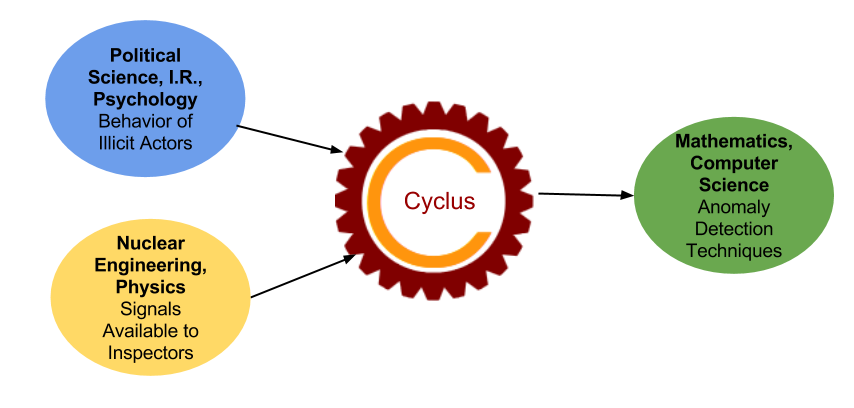
\includegraphics[natwidth=162bp,natheight=227bp, scale=0.45]{./figs/cyclus_interdiscipline.png}
\end{center}
\caption{The \Cyclus nuclear fuel cycle simulator provides a testbed to integrate innovations in treaty verification across many disciplines.}
\label{fig:cyclus_diagram}
\end{figure}

An effective treaty verification regime must synthesize knowledge from the realms of political science, international relations, nuclear physics and engineering, and even behavioral psychology.  Figure \ref{fig:cyclus_diagram} illustrates  the role of a fuel cycle simulator such as \Cyclus in bringing together these disparate fields to provide insights into proposed verification technologies. A fuel cycle simulator tracks the flow of nuclear material through the facilities in a fuel cycle\cite{huff_fundamental_2016}.  Uranium enrichment and spent fuel reprocessing are two particularly sensitive parts of the fuel cycle, but correlated signatures of illicit activity are likely to be present across the fuel cycle. A fuel cycle simulator creates synthetic data, such as what would be available to an inspector, for many different facilities simultaneously while incorporating a system-level perspective of proliferation scenarios. This synthetic data can then be used as a testbed to investigate the efficacy of new detection and analysis techniques. In this way, simulators can be used to  to illucidate the strengths and weaknesses of various verification strategies.